\subsection{Fuzzy C-Means}

We selected the \textbf{generalized suppressed Fuzzy C-Means} (gs-FCM) algorithm, an improvement over traditional FCM, which often shows multimodal behavior near cluster boundaries (Fig. \ref{fig:FCMIP}). This issue, where fuzzy memberships remain high for unrelated clusters, was addressed by Höppner and Klawonn \cite{Hoppner2003}.

The suppressed Fuzzy C-Means (s-FCM) algorithm \cite{Fan2003} enhances convergence speed and classification accuracy without minimizing the traditional objective function \( J_{\text{FCM}} \). It introduces a suppression step during each iteration to reduce non-winner fuzzy memberships, which is mathematically equivalent to virtually reducing the distance to the winning cluster's prototype (Fig. \ref{fig:VirtualReduction}) \cite{Szilagyi2010}.

Szilágyi et al. \cite{Szilagyi2010} defined the quasi-learning rate \(\eta\) of s-FCM, analogous to learning rates in competitive algorithms:
\[
\eta(m, \alpha, u_{wk}) = 1 - \frac{\delta_{wk}}{d_{wk}} = 1 - \left( 1 + \frac{1-\alpha}{\alpha u_{wk}} \right)^{(1-m)/2}.
\]

Building on this, gs-FCM modifies the learning rate to decay linearly with increasing winner membership \(u_{wk}\) for faster convergence, as proposed in $sg_\rho$-FCM \cite{Szilagyi2014}:
\[
\eta(u_{wk}) = 1 - \rho u_{wk}, \quad \text{where } 0 \leq \rho \leq 1.
\]
This approach ensures a logical adaptation of membership weighting, expressed as:
\[
\alpha_k = \left[ 1 - u_w + u_w \left( 1 - f(u_w) \right)^{2/(1-m)} \right]^{-(1-m)}.
\]

\begin{figure}[htbp]
    \centering
    \begin{subfigure}{0.45\textwidth}
        \centering
        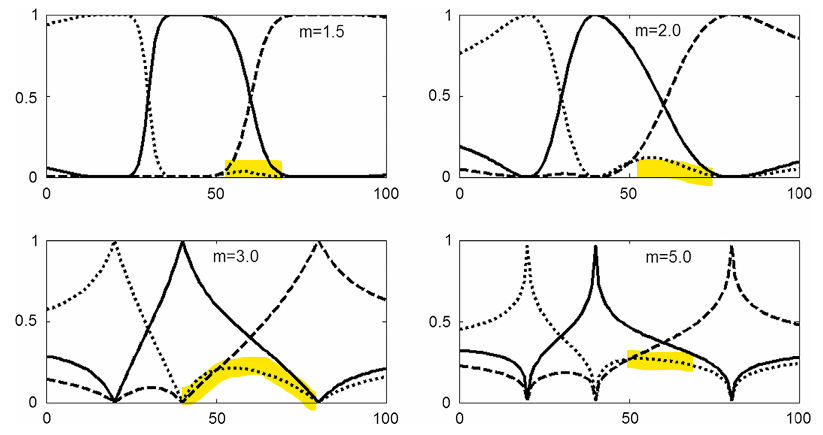
\includegraphics[width=\linewidth]{figures/FCMIP}
        \caption{Multimodal fuzzy memberships near cluster boundaries for varying fuzzy exponent \(m\).}
        \label{fig:FCMIP}
    \end{subfigure}
    \hfill
    \begin{subfigure}{0.45\textwidth}
        \centering
        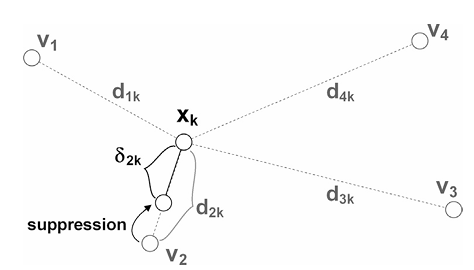
\includegraphics[width=\linewidth]{figures/s-FCM}
        \caption{Suppression effect: Winner cluster (\(w_k=2\)) gains increased membership while non-winners are suppressed.}
        \label{fig:VirtualReduction}
    \end{subfigure}
    \caption{Figures adapted from \cite{Szilagyi2014}.}
\end{figure}
